\documentclass[12pt, twoside]{article}
\usepackage[francais]{babel}
\usepackage[T1]{fontenc}
\usepackage[latin1]{inputenc}
\usepackage[left=5mm, right=5mm, top=3mm, bottom=3mm]{geometry}
\usepackage{float}
\usepackage{graphicx}
\usepackage{array}
\usepackage{multirow}
\usepackage{amsmath,amssymb,mathrsfs}
\usepackage{textcomp}
\pagestyle{empty}
\usepackage{soul}

\begin{document} 


\begin{flushleft}
NOM PRENOM: \ldots \ldots \ldots \ldots \ldots \ldots \ldots \ldots \ldots
 \end{flushleft}


\begin{center}
{\fbox{$4^{e}4$ \qquad \qquad \textbf{\Large{Devoir surveill� 3}}
\qquad \qquad 23/01/2015}}
\end{center}


 
\enskip



\ul{\textbf{Exercice 1:}} \textit{(4,5 points)} Pour cet exercice, on ne
demande pas de justification.

\begin{tabular}{ccc}
\begin{minipage}{6cm}
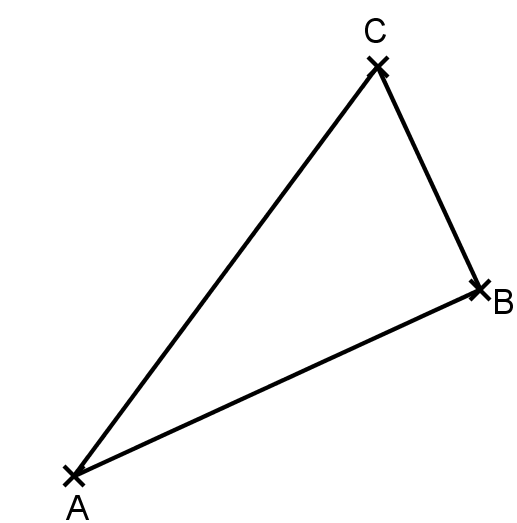
\includegraphics[width=35mm]{images/ex11.png}


\end{minipage}
&
\begin{minipage}{6cm}
\begin{center}
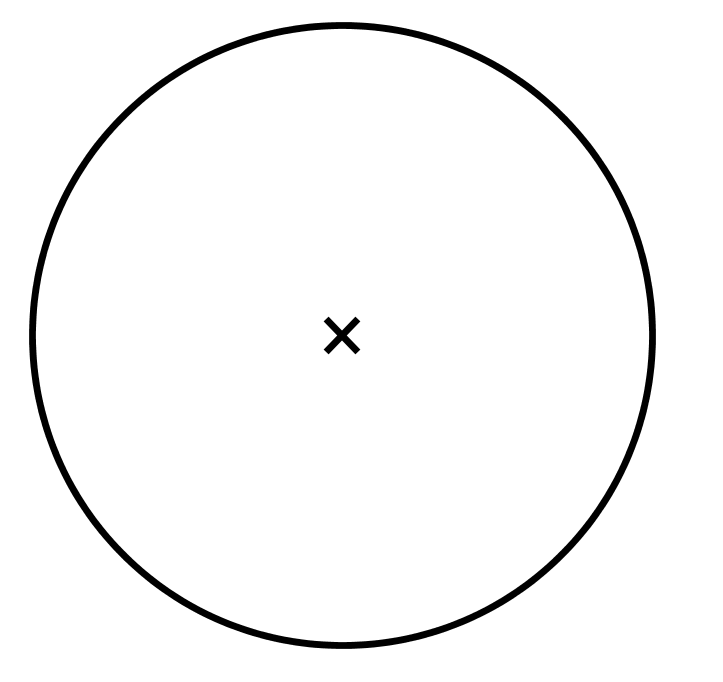
\includegraphics[width=35mm]{images/ex12.png}
\end{center}

\end{minipage}
&
\begin{minipage}{6cm}
\begin{center}
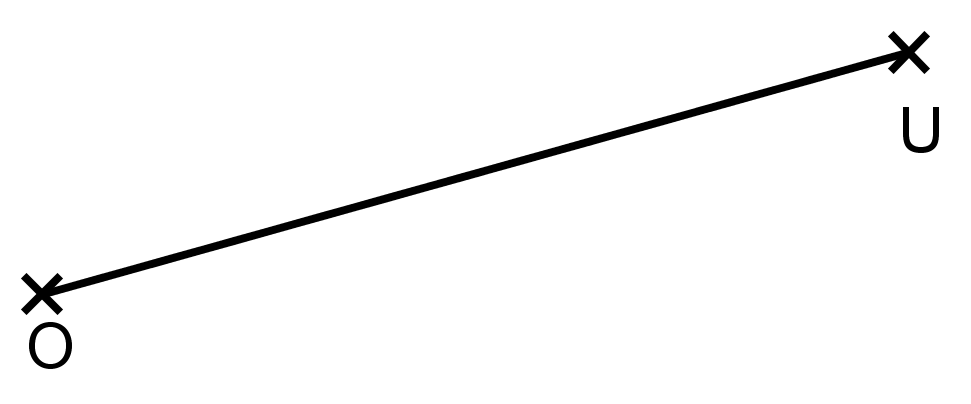
\includegraphics[width=35mm]{images/ex13.png}
\end{center}


\end{minipage} \\

\begin{minipage}{6cm}
1. Construire le cercle circonscrit 

au triangle ABC.
\end{minipage}
&
\begin{minipage}{6cm}
2. Construire un triangle DEF 

inscrit dans le cercle rectangle 

en D.
\end{minipage}
&
\begin{minipage}{6cm}
3. Construire un triangle OUI 

rectangle en I tel que UI=3cm.
\end{minipage}
\end{tabular}

 
\bigskip

\bigskip

\ul{\textbf{Exercice 2:}} \textit{(3 points)}

\begin{tabular}{cc}
\begin{minipage}{11cm}
\begin{enumerate}
  \item D�montrer que le triangle DEF est rectangle en D.
  \item Calculer DJ. Justifier votre r�ponse.
\end{enumerate}
\end{minipage}
&
\begin{minipage}{8cm}
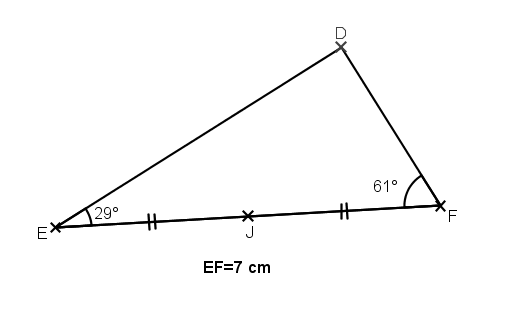
\includegraphics[width=6cm]{images/ex4.png}
\end{minipage}
\end{tabular}


\bigskip

\bigskip

\ul{\textbf{Exercice 3:}} \textit{(4 points)}


\begin{tabular}{cc}
\begin{minipage}{12cm}
\begin{enumerate}
  \item Quel est le centre du cercle circonscrit du triangle KOU? Justifier
  votre r�ponse.
  \item En d�duire que les points O, K, L et U appartiennent � un m�me
  cercle. Justifier votre r�ponse.
\end{enumerate}
\end{minipage}
&
\begin{minipage}{6cm}
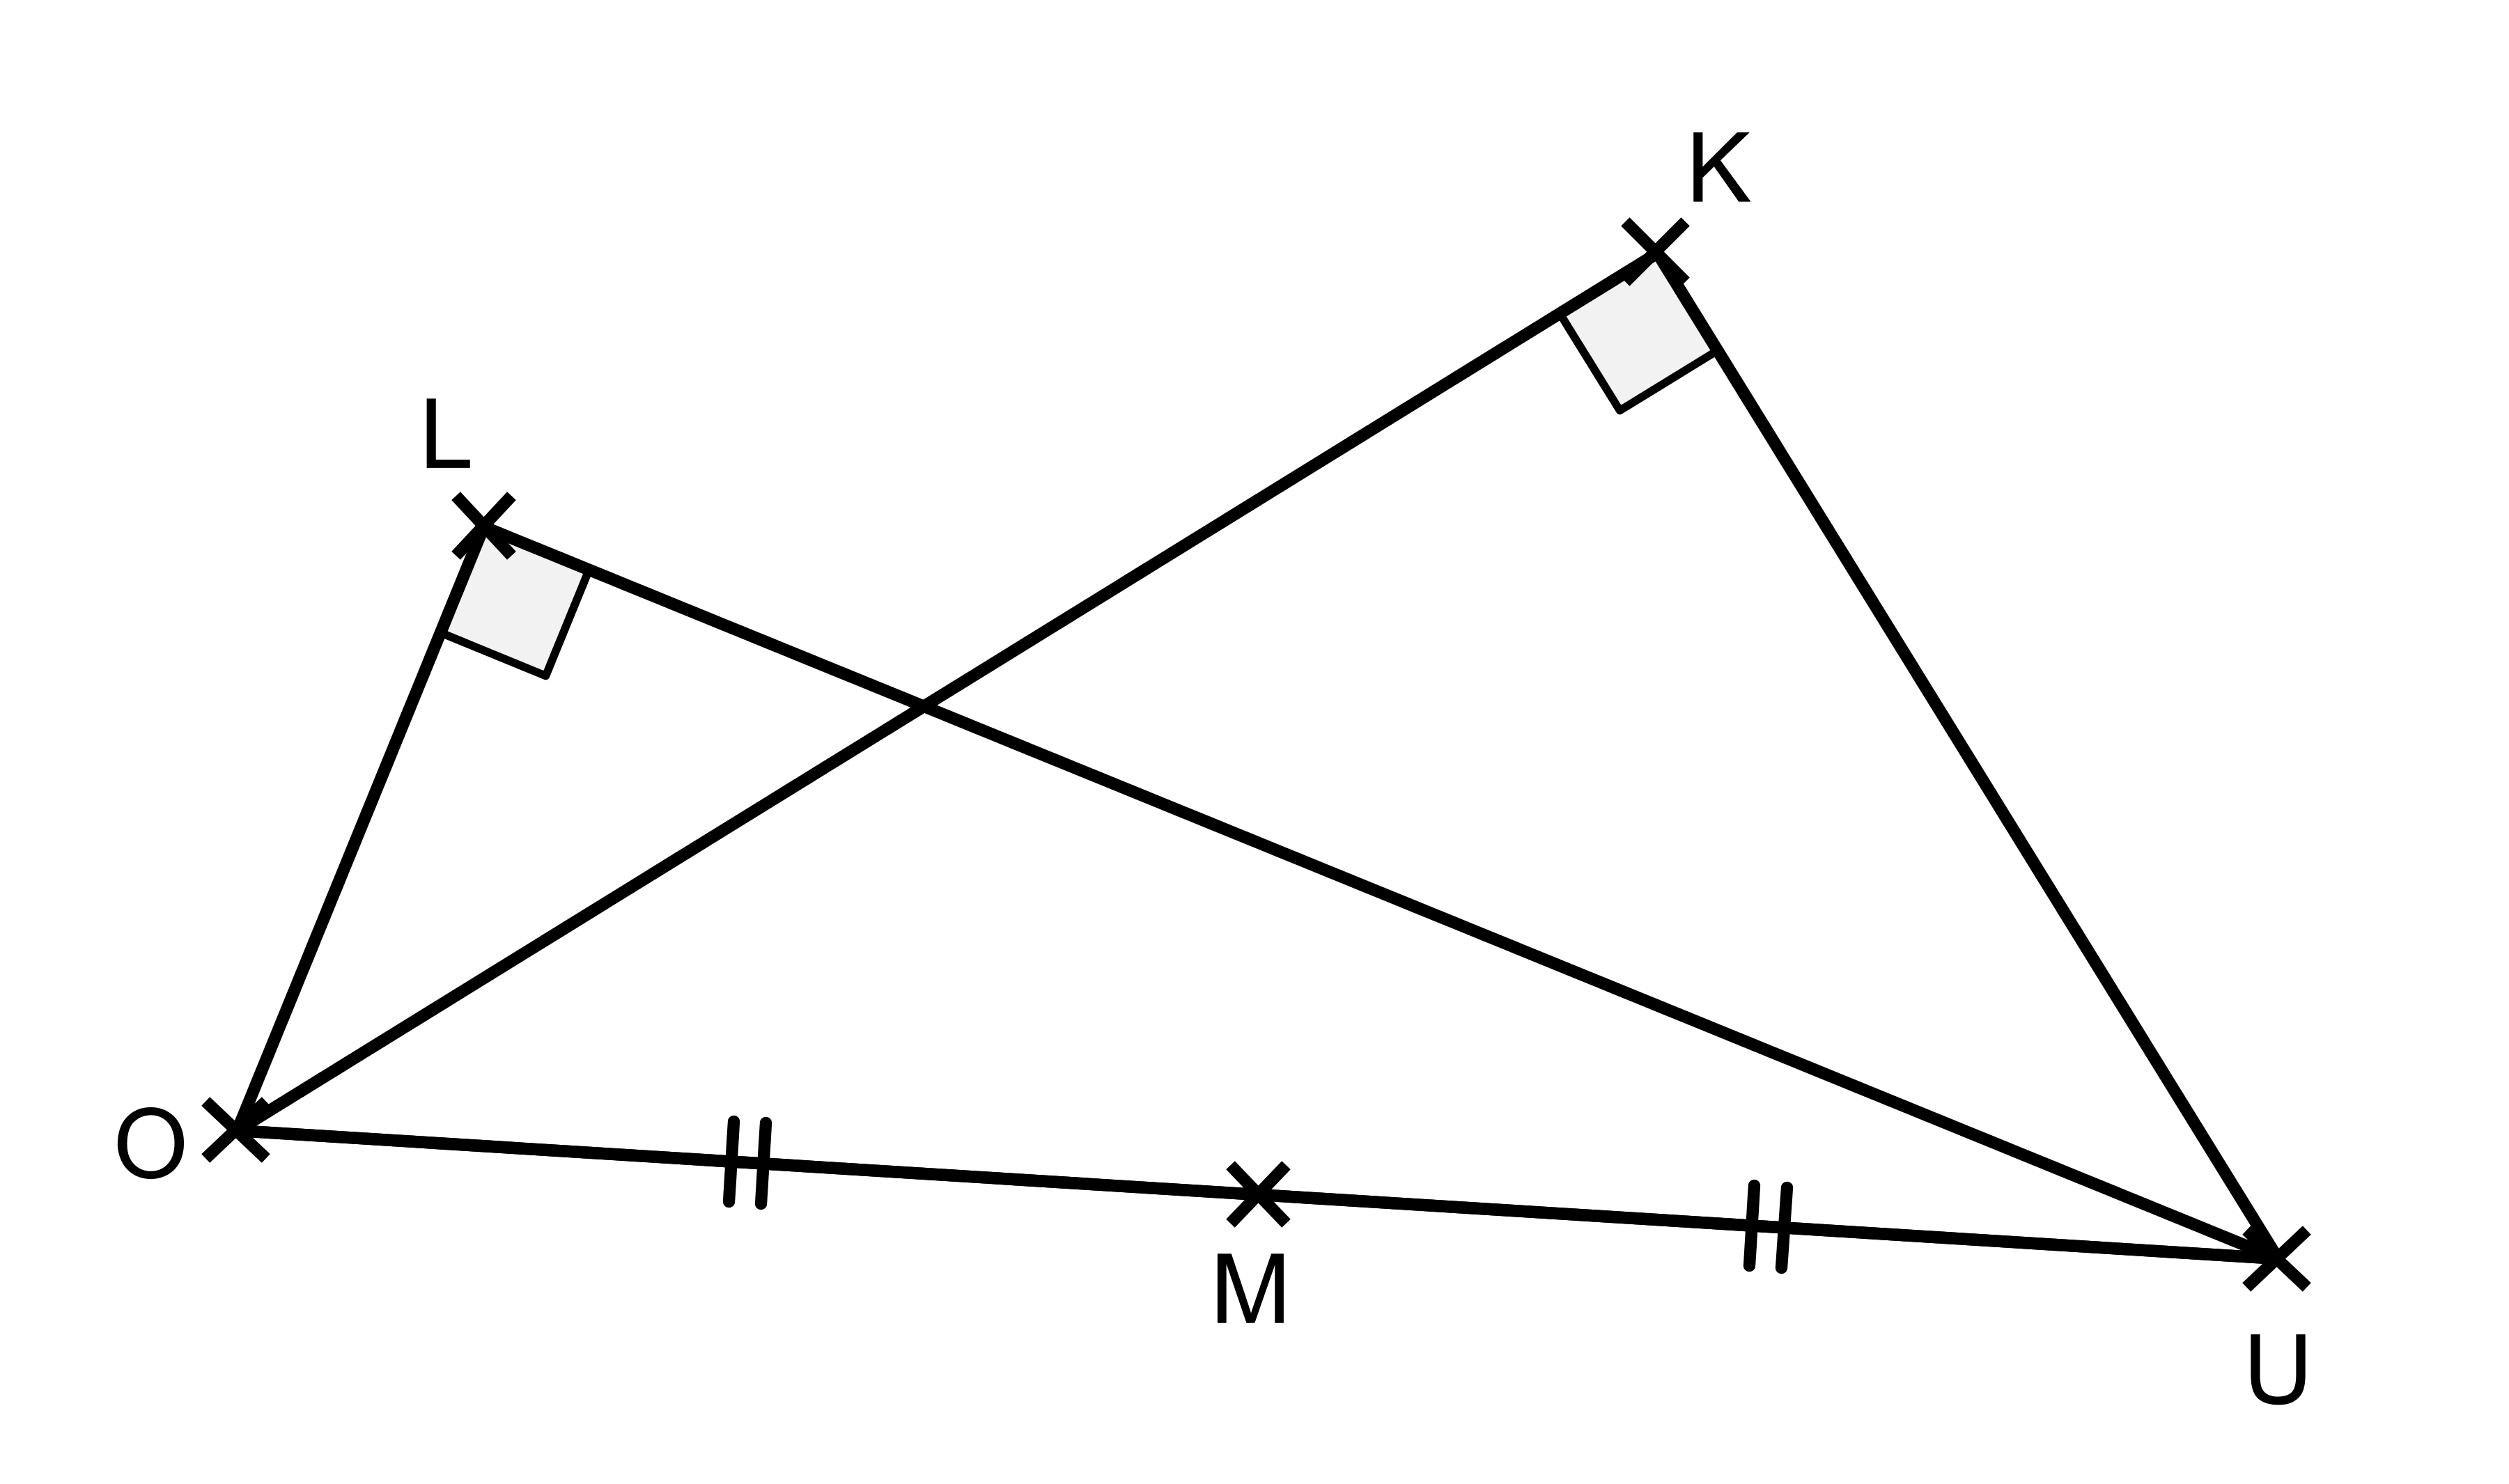
\includegraphics[width=5cm]{images/ex5.png}
\end{minipage}
\end{tabular}

\bigskip


\bigskip

\ul{\textbf{Exercice 4:}} \textit{(5,5 points)}


\begin{tabular}{cc}
\begin{minipage}{12cm}
\begin{enumerate}
  \item Quelle est la nature du triangle ABC? Justifier votre r�ponse.
  \item Calculer AB. Justifier votre r�ponse.
  \item En d�duire le p�rim�tre et l'aire du triangle ABC.
\end{enumerate}
\end{minipage} 
&
\begin{minipage}{6cm}
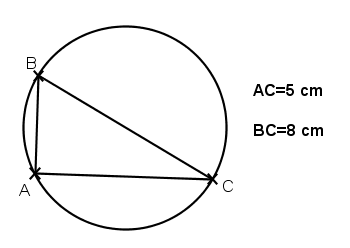
\includegraphics[width=5cm]{images/ex6.png}
\end{minipage}
\end{tabular}


\bigskip

\bigskip


\ul{\textbf{Exercice 5:}} \textit{(3points)}

\begin{tabular}{cc}
\begin{minipage}{10cm}
Construire la perpendiculaire � la droite $(d)$ passant par A puis la
perpendiculaire � la droite $(d)$ passant par B sans utiliser l'�querre.

\bigskip

Expliquer votre d�marche.
\end{minipage}  
& 
\begin{minipage}{8cm}
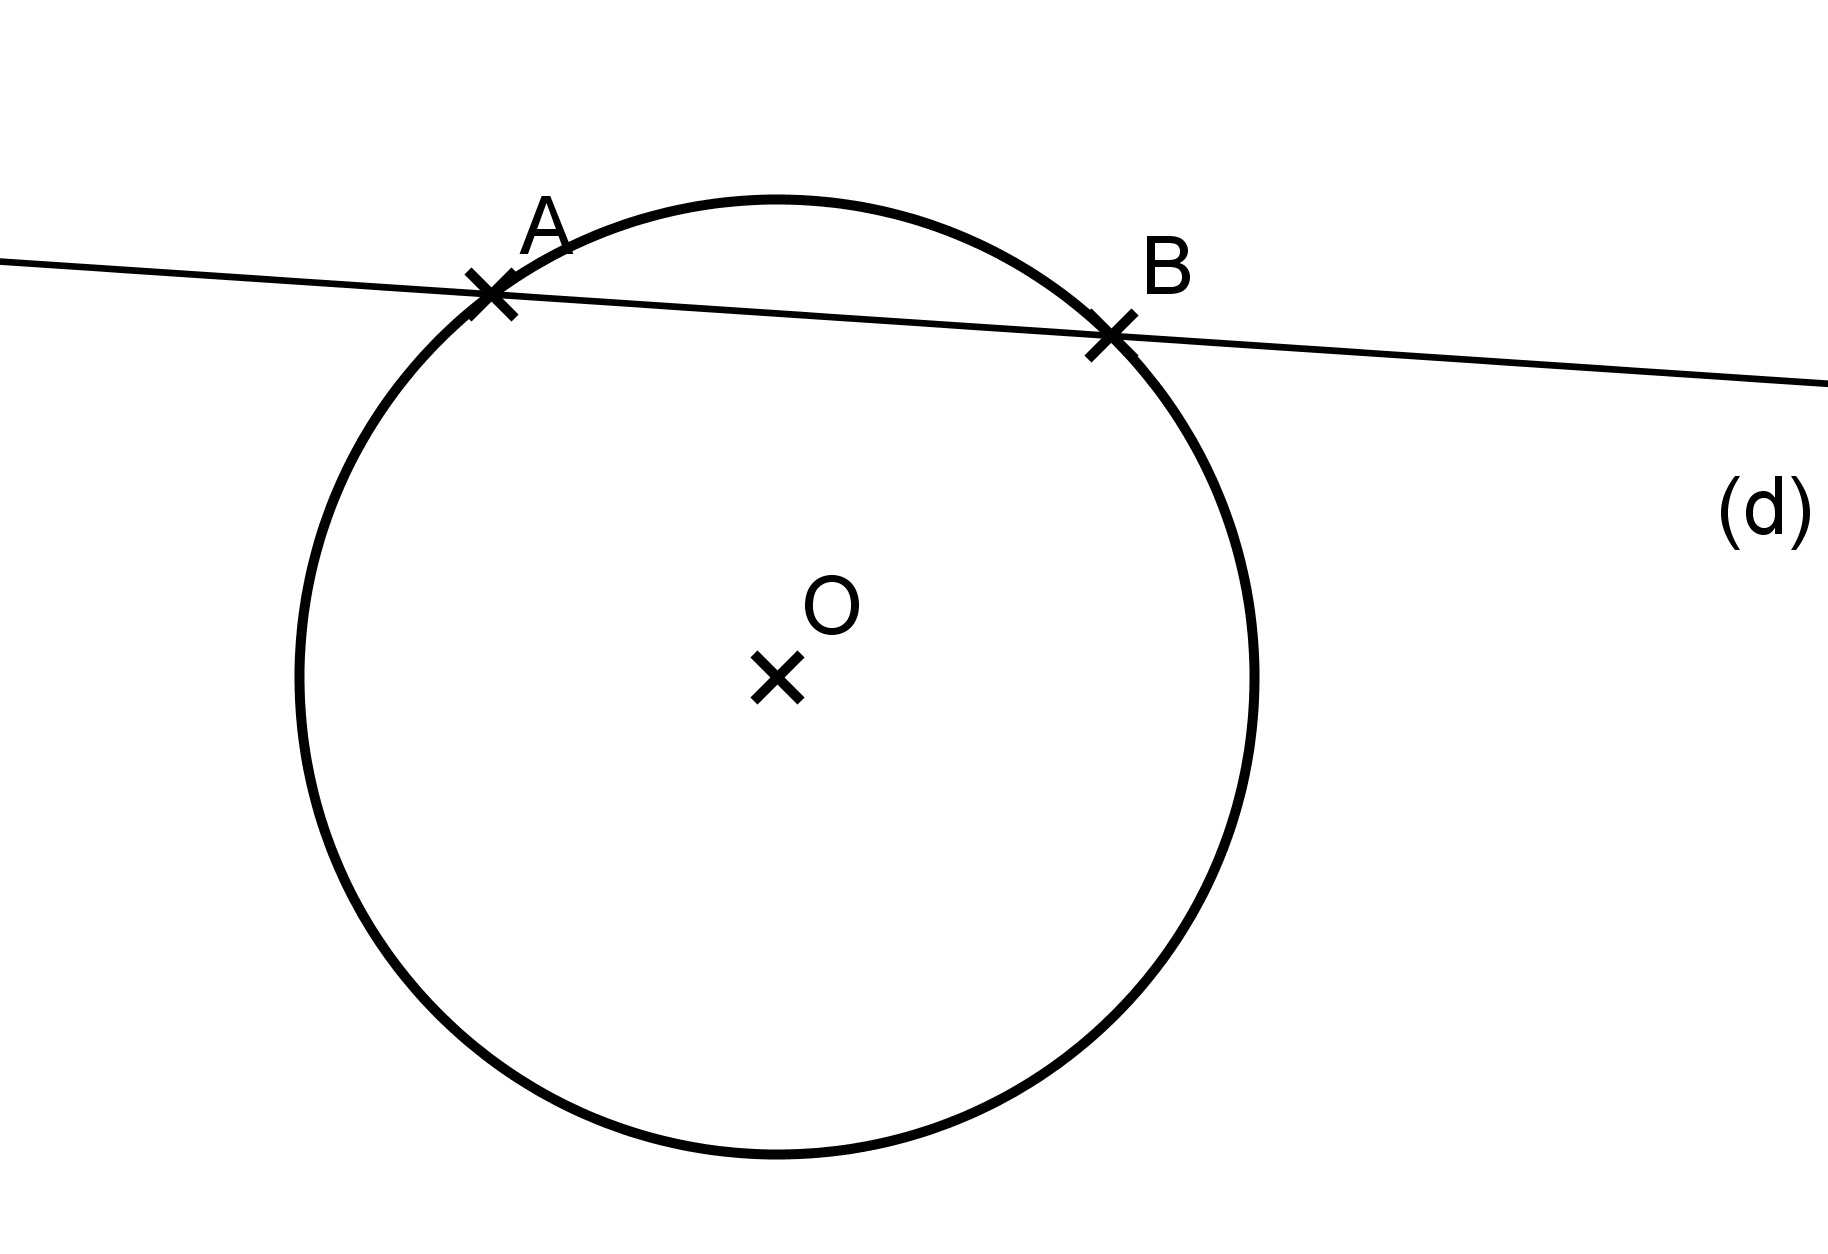
\includegraphics[width=6cm]{images/construction.png}
\end{minipage}
\end{tabular}


\end{document}
